\cotefile{37}
\scanpage{52}
\noindent SGA 5 \(\overline{\underline{\mathrm{VII}}}\)\quad th de Lefschetz faible sans supposer \(X\) ni \(Y\) lisses (seulement \(X-Y\) lisse \ldots)

\noindent SGA 5 \(\overline{\underline{\unsure{\mathrm{V}|\mathrm{VI}}}}\)\quad \(\mathbb{Q}_{\ell}\)-faisceau : \unsure{rajouter} définition \unsure{raisonnable} en termes de \uline{champ} \uline{associé}

\noindent SGA 5. \(\deleted{\overline{\underline{\unsure{\mathrm{IV}|\mathrm{V}|\mathrm{VI}}}}}\)\,\inserted{\tikz[baseline=(vi.base)]{\node[inner sep=1pt] (vi) {\(\overline{\underline{\mathrm{VI}}}\)};\draw[thin] ([xshift=-1pt,yshift=1pt]vi.north west) .. controls +(270:0.6cm) and +(265:0.6cm) .. ([xshift=3pt,yshift=3pt]vi.north east);}}\quad Reprendre en langage de \(\mathbb{Z}_{\ell}\)-\unsure{faisceaux|faisceau} ou\textsuperscript{\inserted{\unsure{+|*}}} \(\mathbb{Q}_{\ell}\)-faisceaux les notions essentielles dont il a été question dans SGA 4 (\unsure{,|.} Ajouter nouveau N\textsuperscript{\uline{o}}).

\noindent SGA 5 \(\overline{\underline{\mathrm{IV}}}\)\quad Essayer de faire dans le cas relativement lisse ttes les constructions essentielles

\figure{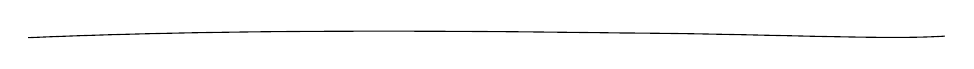
\begin{tikzpicture}[x=\linewidth,y=1cm]
\draw[thin] (0,0) .. controls (.23,.12) and (.49,.08) .. (.62,.06)
 .. controls (.77,.05) and (.90,-.03) .. (.96,.02);
\end{tikzpicture}}

\noindent \(\overline{\underline{\mathrm{VI}}}\)\quad \unsure{Systèmes|Système} projectifs \inserted{\tikz[baseline=(adiques.base)]{\node[inner sep=0pt] (adiques) {\unsure{adiques}};\draw[thin] ([xshift=-0.35em,yshift=-0.7ex]adiques.south west) .. controls +(85:1.2ex) and +(-1em,-0.15ex) .. (adiques.south) .. controls +(0.8em,0.15ex) and +(0em,-0.7ex) .. ([xshift=0.12em,yshift=0.1ex]adiques.east);}} dans les catégories \unsure{dérivées} \ldots\ (ou dans thèse)\margin{\unsure{:}}

\noindent SGA 5 \(\mathrm{V}\)\quad dans introduction du livre ou de l'exposé signaler l'ennui des coeff. trop particuliers \((\mathbb{Z}_{\ell},\,\mathbb{Z}/\ell^{\unsure{n|\nu}}\mathbb{Z}\ \unsure{-\,-|\ldots})\)

\figure{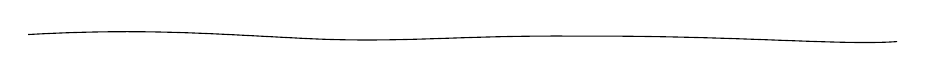
\begin{tikzpicture}[x=\linewidth,y=1cm]
\draw[thin] (0,.03) .. controls (.12,.11) and (.19,.04) .. (.29,-.02)
 .. controls (.39,-.08) and (.45,.02) .. (.57,.01)
 .. controls (.74,.02) and (.85,-.11) .. (.91,-.06);
\end{tikzpicture}}

\noindent \(\mathrm{I}\)\quad \S\ 5\qquad Donner, si \(i\unsure{{:}|{<}|{\in}}\unsure{\eta|y}\longrightarrow X\) inclusion du \(\mathrm{pt}\) générique, et \(F_{\eta}\) Module loc. libre sur \(\eta\)
\[
 D\bigl(i_{*}(F_{\eta})\bigr)=i_{*}\bigl(D(F_{\eta})\bigr)
\]
% archive sheet number: 51
\clearpage
\scanpage{53}
% letterhead
\begin{center}
{\sffamily INSTITUT\\
DES HAUTES ÉTUDES SCIENTIFIQUES}\\[-0.4ex]
\rule{1.7cm}{0.5pt}
\end{center}

\noindent SGA 5\qquad \(\overline{\underline{\mathrm{XIII}}}\)

\figure{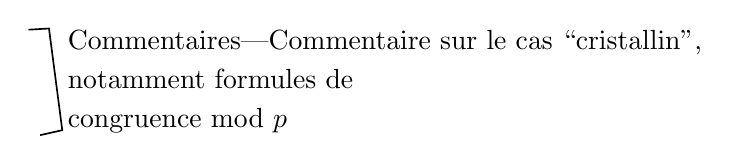
\begin{tikzpicture}
\node[anchor=west,inner sep=0pt,align=left] (lignes) {\unsure{Commentaires|Commentaire} sur le cas ``cristallin'',\\[0.5ex]
notamment formules de\\[0.5ex]
congruence \(\mathrm{mod}\ p\)};
\draw[semithick] ([xshift=-1.4em]lignes.north west) --
 ([xshift=-0.66em,yshift=0.1ex]lignes.north west) --
 ([xshift=-0.18em,yshift=0.30ex]lignes.south west) --
 ([xshift=-0.98em,yshift=-0.12ex]lignes.south west);
\end{tikzpicture}}

\noindent \deleted{\illegible{1}}\quad \(\overline{\underline{\mathrm{IV}}}\)\qquad Faire attention au cas relatif, consulter \(\overline{\underline{\mathrm{VII}}}\) et SGA 6 \(\overline{\underline{\mathrm{X}}}\)

\noindent \(\overline{\underline{\mathrm{XIV}}}\)\quad (\unsure{Problèmes} et \unsure{Commentaires|Commentaire})

Signaler les variantes \(\mathrm{mod}\ p\) et \unsure{variantes|Variantes} cristallines (cf \unsure{mes|une} \unsure{notes|note} à propos th. de Katz).
% archive sheet number: 52
\clearpage
\scanpage{54}
% letterhead
\begin{center}
{\sffamily HARVARD UNIVERSITY\\
CAMBRIDGE, MASSACHUSETTS 02138}
\end{center}
% upper right, boxed in pencil
\margin{\figure{\tikz[baseline=(copie.base)]{\node[align=left,inner sep=2pt] (copie) {Faire copie\\pour \unsure{Jouanolou}};\draw[thin] (copie.north west) -- (copie.north east) -- ([yshift=-2pt]copie.north east);\draw[thin] ([yshift=-1pt]copie.north west) -- (copie.south west) -- (copie.south east) -- ([yshift=-5pt]copie.north east);}}}
% letterhead
\noindent {\sffamily DEPARTMENT OF MATHEMATICS\\
2 DIVINITY AVENUE}\\
\hfill Aug 4, 1969\\

\noindent Dear Grothendieck,\\

I have been reading recently some notes from the IHES (one of your seminars, I suppose) entitled ``Exposé \(\overline{\underline{\mathrm{V}}}\). Systèmes
\reversemarginpar\margin{\hfill\rule{0.4pt}{1.6\baselineskip}}\normalmarginpar%
projectifs J-adiques, par J.P. Jouanolou.'' Could you tell me (for purposes of reference) to which seminar they belong, and whether there is a more recent edition?

Also I have some comments and questions. The most serious question is that I do not understand the proof of the ``Theorem of Shih'', \unsure{A.3.1|A.3.1.} on page 46. It seems to me that the lemma on p. 45 is valid only for \(r>p\) (cf EGA \(\unsure{0|O}_{\overline{\underline{\mathrm{III}}}}\) 13.5.5.2), and so \deleted{\unsure{the|from}} the equivalence of statements (i) and (ii) of the theorem is not clear. (I do agree, however, with the weaker statement ``(resp.\ldots)'' in parentheses). This casts doubt on the following theorem A.3.2 on p. 47, and also on the earlier Prop. 5.3.1 on p. 40\unsure{.|,} These difficulties would disappear if one worked \unsure{throughout} in the category \(\mathrm{pro}\text{-}A\) \margin{\unsure{:}} of projective systems with the usual equivalence, rather than in the \deleted{category} finer category \(P_{AR}\).

Other comments: p. 42 line \(\unsure{\dot{-}|{-}}1\). Isn't the spectral sequence actually biregular in case of a finite filtration?

p. 47 line \(-1\). I think the hypothesis should be stated for \(n\) and \(n+1\), instead of \(n\) and \(n-1\) (cf EGA \(0_{\overline{\underline{\mathrm{III}}}}\) 11.1.10).
% archive sheet number: 53
\clearpage
\scanpage{55}
\mspage{2}

\noindent p. 38\quad I believe the artinian hypothesis in this proposition is unnecessary, if one assumes that \(X\) and \(Z\) are both \inserted{AR}-\(J\)-adic noetherian. To be precise, let

% The two text rows occupy the same cells spanned by the three upward arrows.
\diagram{\begin{tikzcd}[ampersand replacement=\&,column sep=1em,row sep=0.6ex]
0 \arrow[r] \& X \arrow[r] \& Y \arrow[r] \& Z \arrow[r] \& 0\\
\&\& \makebox[0pt][c]{\parbox{0.96\linewidth}{\raggedright
be an exact sequence of projective systems of \(A\)-modules, such that
\(J^{n+1}X_n=J^{\unsure{n+1|n+{}}}Y_n=J^{n+1}Z_n=0\) for all \(n\), and assume \(X\) and \(Z\) are AR-\(J\)-adic noetherian. Then \(Y\) is also AR-\(J\)-adic noetherian.\par
\smallskip\noindent Indeed, taking \(\underset{\longleftarrow}{\lim}\) we get an exact sequence}} \&\&\\
0 \arrow[r] \& M' \arrow[r] \& M \arrow[r] \& M'' \arrow[r] \& 0\\
\&\& \makebox[0pt][c]{\parbox{0.96\linewidth}{\raggedright
of \(A\)-modules, with \(M',M''\) finite type, so \(M\) is also finite type.
let \(\mathbb{A}\) be the projective system \((A/J^{n+1})_n\). Then by Artin-Rees, we have an exact sequence}} \&\&\\
0 \arrow[r] \& M'\otimes\mathbb{A} \arrow[r] \arrow[uuuu,thin,start anchor=north east,end anchor=south west,bend left=4] \&
M\otimes\mathbb{A} \arrow[r] \arrow[uuuu,thin,start anchor=north east,end anchor=south,bend left=3] \&
M''\otimes\mathbb{A} \arrow[r] \arrow[uuuu,thin,start anchor=north east,end anchor=south east,bend left=2] \& 0
\end{tikzcd}}

\noindent in the category \(P_{AR}\) of projective systems up to translation. There is a natural map of this sequence to the first. The two outside arrows are isomorphisms, so \(M\otimes\mathbb{A}\xrightarrow{\approx}Y\), which \unsure{shews|shows} that \(Y\) is AR-\(J\)-adic.

I came to these questions while \deleted{\illegible{1}} working on my paper ``Affine Duality and Cofiniteness'' which I am finally preparing for publication. \margin{\unsure{:}}I will send you a copy when it is ready.

\noindent\hfill Sincerely yours,\\
\null\hfill R. Hartshorne\\
% archive sheet number: 54
\clearpage
\scanpage{75}
% slanted
\reversemarginpar\margin{\shortstack[l]{\unsure{joindre}\\SGA 7 \(\overline{\underline{\mathrm{VI}}}\) ?\\App. \(\overline{\underline{\mathrm{II}}}\)}}\normalmarginpar
\noindent\hfill Bures sur Yvette, le 21 octobre 1968\\

\noindent Cher Grothendieck,\\

En fait, il n'est pas nécessaire de faire de savants recollages de complexes cotangents pour prouver que

\noindent \uline{proposition} : \uline{Soit} \(X\) \uline{un espace analytique complexe compact}. \uline{Pour que} \(X\) \uline{soit un schéma}, \uline{il faut et suffit que} \(X_{\mathrm{red}}\) \uline{le soit}

On se ramène à \deleted{supposer} montrer que si \(X_0\) est défini par un Idéal de carré nul, soit \(\mathscr{N}\), de \(X\), alors
\[
 (X_0\text{ est un schéma})\ \Longrightarrow\ (X\text{ est un schéma})
\]

Soit \(E^{\mathrm{an}}(X_0,\mathscr{N})\) et \(E^{\mathrm{alg}}(X_0,\mathscr{N})\) les groupes analytiques et algébriques d'extensions infinitésimales de \(X_0\) par \(\mathscr{N}\). Soit enfin \(\unsure{K|\mathbb{K}}\) le complexe cotangent de \(X_0\), \uline{donné localement, dans la catégorie dérivée}. il s'obtient en plongeant \uline{localement} (Zariski, ou étale) \(X_0\) dans un \unsure{schéma} lisse \ldots\ et permet de définir
\begingroup
\makeatletter\tagsleft@true\makeatother
\[
 \mathscr{H}om(K,\mathscr{N})\qquad\text{et}\qquad\mathscr{E}xt^{1}(K,\mathscr{N})\ .\tag*{(1)}
\]
\endgroup

Soit le diagramme :

\diagram{\footnotesize
\begin{tikzcd}[ampersand replacement=\&,column sep=0.85em,row sep=1.6em]
 (2) \& 0 \arrow[r] \&
 H^{1^{\mathrm{alg}}}(X_0,\mathscr{H}om(K,\mathscr{N})) \arrow[r] \arrow[d] \&
 E^{\mathrm{alg}}(X_0,\mathscr{N}) \arrow[r,"\alpha"] \arrow[d] \&
 H^{0}(X_0,\mathscr{E}xt^{1}(K,\mathscr{N})) \arrow[d] \\
 \& 0 \arrow[r] \&
 H^{1^{\mathrm{an}}}(X_0,\mathscr{H}om(K,\mathscr{N})) \arrow[r] \&
 E^{\mathrm{an}}(X_0,\mathscr{N}) \arrow[r,"\beta"] \&
 H^{0^{\mathrm{an}}}(X_0,\mathscr{E}xt^{1}(K,\mathscr{N}))
\end{tikzcd}}
\margin{\unsure{:}}

Vu les significations (locales) de (1), les lignes sont exactes ; par GAGA, les flèches verticales extrêmes sont des isomorphismes. Reste à \deleted{comparer les images de \mbox{\(\alpha\)} et \mbox{\(\beta\)}} montrer que \(\operatorname{Im}(\beta)\subset\operatorname{Im}(\alpha)\).
% archive sheet number: 74
\clearpage
\scanpage{76}
\noindent Soit donc \(U_i\) un recouvrement affine de \(X_0\), et
\[
 e\in H^{0^{(\mathrm{alg})}}(X_0,\mathscr{E}xt^1(K,\mathscr{N}))
\]
représenté par des classes d'isomorphies (algébriques) d'extensions \(\inserted{U'_i}\) de \(U_i\) par \(\mathscr{N}\mid U_i\), classes d'isomorphies qui se recollent :

\[
 \text{soit }\unsure{\eta|n|\gamma}_{ij}\text{ un isomorphisme}\qquad
 U'_{\unsure{j|i}}\mid U_i\cap U_j
 \xrightarrow{\sim}
 U'_{\unsure{i|j}}\mid U_i\cap U_j\ .
\]

L'obstruction à construire des \(\eta_{ij}\) \deleted{\unsure{d}}tels que \(\eta_{ij}\eta_{jk}=\eta_{ik}\) est \unsure{donné|donnée} par \(d_2\eta\) où \(d_2\) est une certaine flèche
\[
 d_2:H^0(X_0,\mathscr{E}xt^1(K,\mathscr{N}))\longrightarrow
 H^2(X_0,\mathscr{H}om(K,\mathscr{N}))
\]

La même construction marche dans le cas analytique, et on conclut par une nouvelle application de GAGA.

\uline{Rmq} \unsure{1|s} : \unsure{itou} pour les espaces algébriques, espaces rigides analytiques ; schémas formels

\deleted{\uline{\unsure{Rmq 2|Rmqs}}} :

\noindent\hfill Bien à toi\\
\null\hfill P. Deligne\\
\margin{\unsure{:}}
% archive sheet number: 75
\clearpage
\scanpage{77}
% letterhead
\begin{center}
{\sffamily INSTITUT\\
DES HAUTES ÉTUDES SCIENTIFIQUES}\\[-0.4ex]
\rule{1.7cm}{0.5pt}
\end{center}

\figure{\footnotesize\begin{tikzpicture}
\node[anchor=west,inner sep=0pt,align=left] (haut) at (0,0) {
\(\overline{\underline{\unsure{\mathrm{VI}|\mathrm{VII}}}}\,
 1.11\ \text{\unsure{à|:}}\ 1.14\
 \text{\unsure{apres|après}}\ 1.15\,-\,\unsure{1.22|1.21}\ \text{? Refaire }1.14\ \text{?}\)\\[1.3ex]
\(\overline{\underline{\mathrm{VI}}}\)\quad \unsure{appendice} : lettre Deligne 2 pages};
\draw[semithick] ([xshift=-.15em,yshift=.18ex]haut.north west)
 .. controls +(-.29em,-.26ex) and +(.12em,.50ex) .. ([xshift=-.28em,yshift=.79ex]haut.west)
 .. controls +(.12em,-.62ex) and +(.26em,.22ex) .. ([xshift=-.64em]haut.west)
 .. controls +(.49em,-.17ex) and +(.05em,.44ex) .. ([xshift=-.26em,yshift=-.82ex]haut.west)
 .. controls +(.02em,-.46ex) and +(-.23em,-.13ex) .. ([xshift=-.1em,yshift=-.1ex]haut.south west);
\node[inner sep=0pt] (sga) at ([xshift=-1.15cm,yshift=-.4ex]haut.west) {SGA 7};
\draw[thin] ([xshift=-.79cm,yshift=-.06cm]sga.center)
 .. controls +(.07cm,.45cm) and +(-.47cm,.03cm) .. ([xshift=.72cm,yshift=.64cm]sga.center)
 .. controls +(.04cm,-.47cm) and +(.38cm,.03cm) .. ([xshift=-.18cm,yshift=-.65cm]sga.center)
 .. controls +(-.40cm,0cm) and +(-.05cm,-.24cm) .. ([xshift=-.79cm,yshift=-.06cm]sga.center);
\end{tikzpicture}}

% slanted
\reversemarginpar\margin{\raisebox{-1.4\baselineskip}[0pt][0pt]{\shortstack[l]{faire un\\exposé\\\(\overline{\underline{\mathrm{XXIII}}}\) ?}}}\normalmarginpar
\figure{\footnotesize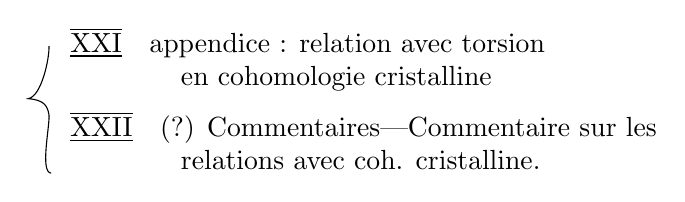
\begin{tikzpicture}
\node[anchor=west,inner sep=0pt,align=left] (bas) at (0,0) {
 \(\overline{\underline{\mathrm{XXI}}}\)\quad \unsure{appendice} : relation avec \unsure{torsion}\\
 \hspace{4em}en \unsure{cohomologie} cristalline\\[1.5ex]
 \(\overline{\underline{\mathrm{XXII}}}\)\quad (?) \unsure{Commentaires|Commentaire} sur les\\
 \hspace{4em}relations avec coh. \unsure{cristalline}.};
\draw[thin] ([xshift=-.75em,yshift=-1.6ex]bas.north west)
 .. controls +(.02em,-1.0ex) and +(.48em,.18ex) .. ([xshift=-1.5em]bas.west)
 .. controls +(.6em,-.12ex) and +(-.06em,.72ex) .. ([xshift=-.75em,yshift=-1.35ex]bas.west)
 .. controls +(.04em,-.9ex) and +(-.42em,.05ex) .. ([xshift=-.67em,yshift=-.25ex]bas.south west);
\end{tikzpicture}}
% archive sheet number: 76
